\documentclass[12pt]{article}

\textwidth 16cm \textheight 23cm \evensidemargin 0cm
\oddsidemargin 0cm \topmargin -2cm
\parindent 0pt
\parskip \medskipamount

\usepackage[utf8]{inputenc}
\usepackage[dutch]{babel}
\usepackage{amssymb}
\usepackage{amsmath}
\usepackage{amsthm}
\usepackage{hyperref}
\usepackage{enumerate}
\usepackage{subfig}
\usepackage{wrapfig}
\usepackage{minibox}
\usepackage{ifthen}
\usepackage{dot2texi}
\usepackage{multicol}
\usepackage{graphicx}
\usepackage{cancel}
%\usepackage{fix-cm}
\usepackage{setspace}
\usepackage{mdframed}
\usepackage{mathtools}
%\usepackage{lipsum}

\usepackage{exsol}
\renewcommand{\exercisename}{}
\renewcommand{\solutionname}{}

\usepackage{fancyhdr}
\pagestyle{fancy}

\usepackage{color}
\newcommand{\todo}[1]{\textcolor{red}{\##1\#}}
\newcommand{\question}[1]{\textcolor{blue}{\##1\#}}

\newcommand{\vraag}[2]{\begin{itemize}\item {\it #1} \vspace*{#2}\end{itemize}}

\newcommand{\degree}{\ensuremath{^\circ}}
\def\LRA{\Leftrightarrow\mkern40mu}

\newcommand\ggd{\qopname\relax o{\mathrm{ggd}}}
\newcommand\kgv{\qopname\relax o{\mathrm{kgv}}}

\newcounter{menucount}\newcounter{curitem}% Counters
\newcommand{\menuitem}{\texttt}% Menu item formatting
\newcommand{\menusep}{\ensuremath{\rightarrow}}% Menu separator
\newcommand{\menuend}{\relax}% Menu end
\newcommand{\menulist}[1]{% \menulist{<menu list>}
  \setcounter{menucount}{0}\setcounter{curitem}{0}% Reset menucount & curitem
  \renewcommand*{\do}[1]{\stepcounter{menucount}}%
  \menulistparser{#1}% Count menu items
  \renewcommand*{\do}[1]{\menuitem{##1}\stepcounter{curitem}\ifnumless{\value{curitem}}{\value{menucount}}{\menusep}{\menuend}}%
  \menulistparser{#1}% Process list
}
\DeclareListParser{\menulistparser}{:}% List separator is ':'

%\graphicspath{{../figuren/}}

\newcommand{\dotrule}[1]{%
   \parbox[t]{#1}{\vspace*{3pt}\dotfill}}
   
\newcommand{\dotFill}{\vspace*{6pt}\dotfill}

\newcommand{\dotlines}[1]{   
\foreach \n in {1,...,#1}{

\vspace*{0.1cm}
\dotfill
\vspace*{0.1cm}
}}

\newcommand{\ruitjes}[1]{

\hskip-2.6cm
\begin{tikzpicture}[scale=1.075,x=1.0cm,y=1.0cm]
\draw [help lines, solid, gray, very thin, step=0.5cm] (0,-#1+0.1cm) grid (21.6,-0.1);
\end{tikzpicture}
\vspace*{-1cm}
}

\newcommand{\ruitjesxy}[2]{
\begin{tikzpicture}[scale=1.01,line cap=round,line join=round,>=triangle 45,x=1.0cm,y=1.0cm]
\draw [color=cqcqcq,dash pattern=on 1pt off 1pt, xstep=0.4.5cm, ystep=0.4.5cm] (0,-#2) grid (#1,0);
\end{tikzpicture}
}

\newcommand{\zrmbox}{\framebox{\phantom{EXE}}\phantom{X}}
\newcommand{\zrm}[1]{\framebox{#1}}

% arule* answerrules
\def\arulefill{\xrfill[-0.5ex]{0.1pt}[lightgray]}
\newcommand{\arules}[1]{
\color{lightgray}
\vspace*{0.10cm}
\foreach \n in {1,...,#1}{
  \vspace*{0.70cm}
  \hrule height 0.1pt\hfill
}\color{black}}
\newcommand{\arule}[1]{
\color{lightgray}{\raisebox{-0.1cm}{\rule[-0.05cm]{#1}{0.1pt}}}\color{black}
}

% environment oefening:
% houdt een teller bij die de oefeningen nummert
% probeert ook de oefening op één pagina te houden
\newcounter{noefening}
\setcounter{noefening}{0}
\newenvironment{oefening}
{
  \stepcounter{noefening}
  \begin{minipage}{\textwidth}
  \vspace*{8pt}{\large\bf Oefening \arabic{noefening}}
}{%
  \end{minipage}
}

% environment voorbeeld:
% houdt een teller bij die de voorbeelden nummert
% nummering herbegint bij elke subsectie
% probeert het voorbeeld op één pagina te houden
\newcounter{nvb}[subsection]
%\@addtoreset{nvb}{subsubsection}
\setcounter{nvb}{0}
\newenvironment{voorbeeld}
{
  \stepcounter{nvb}
  \begin{minipage}{\textwidth}
  \vspace*{4pt}
  \textit{Voorbeeld \arabic{nvb}}\\[5pt]
}{%
  \end{minipage}
}

% environment voorbeeld*:
% probeert het voorbeeld op één pagina te houden
\newenvironment{voorbeeld*}
{
  \begin{minipage}{\textwidth}
  \vspace*{4pt}
  \textit{Voorbeeld}
}{%
  \end{minipage}
}

\newenvironment{onthoud}
{
\begin{mdframed}[nobreak=true,frametitle={Te onthouden}]
}{%
\end{mdframed}
}

\newcommand{\vglproef}[2]{LL= #1\;${=\joinrel=}$\; RL= #2}

\newcommand{\getallenas}[3][1]{
\definecolor{cqcqcq}{rgb}{0.65,0.65,0.65}
\begin{tikzpicture}[scale=#1,line cap=round,line join=round,>=triangle 45,x=1.0cm,y=1.0cm]
\draw [color=cqcqcq,dash pattern=on 1pt off 1pt, xstep=1.0cm,ystep=1.0cm] (#2,-0.2) grid (#3,0.2);
\draw[->,color=black] (#2,0) -- (#3,0);
\draw[shift={(0,0)},color=black] (0pt,2pt) -- (0pt,-2pt) node[below] {\footnotesize $0$};
\draw[shift={(1,0)},color=black] (0pt,2pt) -- (0pt,-2pt) node[below] {\footnotesize $1$};
\draw[color=black] (#3.25,0.07) node [anchor=south west] {$\mathbb{R}$};
\end{tikzpicture}
}

\newcommand{\opdracht}{{\bf Opdracht }}

% geef tabular iets meer ruimte
\setlength{\tabcolsep}{15pt}
\renewcommand{\arraystretch}{1.5}

% geef align iets meer ruimte:
\addtolength{\jot}{0.5em}

\newtheorem{definition}{Definitie}
\newtheorem{eigenschap}{Eigenschap}

\newcommand{\visgraad}[1]{\begin{tabular}{p{0.5cm}|p{#1}}&\\\hline\\\end{tabular}}

\newcommand{\assenstelsel}[5][1]{
\definecolor{cqcqcq}{rgb}{0.65,0.65,0.65}
\begin{tikzpicture}[scale=#1,line cap=round,line join=round,>=triangle 45,x=1.0cm,y=1.0cm]
\draw [color=cqcqcq,dash pattern=on 1pt off 1pt, xstep=1.0cm,ystep=1.0cm] (#2,#4) grid (#3,#5);
\draw[->,color=black] (#2,0) -- (#3,0);
\draw[shift={(1,0)},color=black] (0pt,2pt) -- (0pt,-2pt) node[below] {\footnotesize $1$};
\draw[color=black] (#3.25,0.07) node [anchor=south west] { x};
\draw[->,color=black] (0,#4) -- (0,#5);
\draw[shift={(0,1)},color=black] (2pt,0pt) -- (-2pt,0pt) node[left] {\footnotesize $1$};
\draw[color=black] (0.09,#5.25) node [anchor=west] { y};
\draw[color=black] (0pt,-10pt) node[right] {\footnotesize $0$};
\end{tikzpicture}
}

\newcommand{\ConfigureExSol}{
\renewcommand{\exercisename}{A.C.O.}
\renewcommand{\solutionname}{A.C.O.}
\newcounter{exercise2}[section]
\setcounter{exercise2}{0}
\renewcommand{\theexercise}{%
    \arabic{exercise2}%
}
\renewenvironment{exsol@exercise}[0]
{%
\refstepcounter{exercise2}
  \begin{minipage}[t]{\textwidth}%
    \ifthenelse{\boolean{exsol@exerciseaslist}}
               {\begin{list}%
                   {%
                   }%
                   {%
                     \setlength{\topsep}{0pt}%
                     \setlength{\leftmargin}{1em}%
                     \setlength{\rightmargin}{1em}%
                     \setlength{\listparindent}{0em}%
                     \setlength{\itemindent}{0em}%
                     \setlength{\parsep}{\parskip}}%
                 \item[\hspace*{\leftmargin}\textit{\exercisename{}
                                                    \theexercise:}]
               }%
               {
                 \textbf{\exercisename{} \theexercise:}~
               }
}
{%
  \ifthenelse{\boolean{exsol@exerciseaslist}}
             {\end{list}}{}
  \end{minipage}
  \vspace{1ex}\par
}
}

\onehalfspacing
%singlespacing
%doublespacing



\usepackage{tikz}
\usetikzlibrary{calc,arrows}
\newcommand{\tikzmark}[1]{\tikz[overlay,remember picture] \node (#1) {};}

%%%%%%%%%%%%%%%%%%%%%%%%%%%%%%%%%%%%%%%%%%
% Volgende wijzigingen werden aangebracht tov de originele bis-basis
% * Alles over gemengde getallen heb ik weggelaten, dit is verwarrend met vermenigvuldigen

%%%%%%%%%%%%%%%%%%%%%%%%%%%%%%%%%%%%%%%%%%
% Volgende opmerkingen heb ik nog
% * 

\lhead{}
\rhead{BIS-Basis -- Les 8}

\begin{document}

\ConfigureExSol

\setcounter{section}{7}
\section{Bewerkingen met breuken}

\subsection{Optellen van breuken}

\subsubsection{Gelijknamige breuken}

\begin{minipage}{0.5\textwidth}
\begin{center}
  $$\dfrac{1}{4}$$
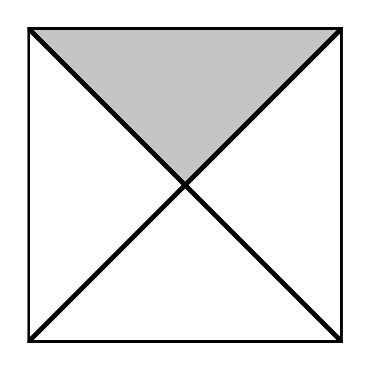
\begin{tikzpicture}[scale=2, line cap=round,line join=round,>=triangle 45,x=1.0cm,y=1.0cm]
\clip(0,0) rectangle (2,2);
\draw [line width=1.6pt] (0,0) -- (0,2) -- (2,2) -- (2,0) -- cycle;
\draw [line width=1.6pt] (0,0) -- (2,0) -- (1,1) -- cycle;
\draw [line width=1.6pt] (2,0) -- (2,2) -- (1,1) -- cycle;
\draw [line width=1.6pt,fill=black,fill opacity=0.23] (1,1) -- (2,2) -- (0,2) -- cycle;
\draw [line width=1.6pt] (0,2) -- (0,0) -- (1,1) -- cycle;
\end{tikzpicture}
\end{center}
\end{minipage}
\begin{minipage}{0.5\textwidth}
\begin{center}
  $$\dfrac{2}{4}$$
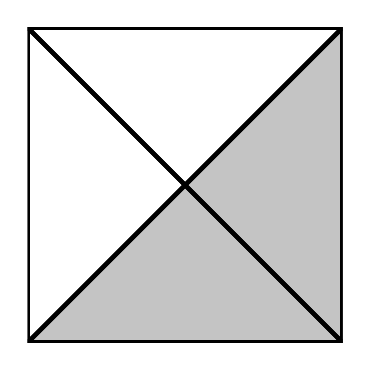
\begin{tikzpicture}[scale=2, line cap=round,line join=round,>=triangle 45,x=1.0cm,y=1.0cm]
\clip(0,0) rectangle (2,2);
\draw [line width=1.6pt] (0,0) -- (0,2) -- (2,2) -- (2,0) -- cycle;
\draw [line width=1.6pt,fill=black,fill opacity=0.23] (0,0) -- (2,0) -- (1,1) -- cycle;
\draw [line width=1.6pt,fill=black,fill opacity=0.23] (2,0) -- (2,2) -- (1,1) -- cycle;
\draw [line width=1.6pt] (1,1) -- (2,2) -- (0,2) -- cycle;
\draw [line width=1.6pt] (0,2) -- (0,0) -- (1,1) -- cycle;
\end{tikzpicture}
\end{center}
\end{minipage}

$\dfrac{1}{4}+\dfrac{2}{4}=\dfrac{3}{4}$, dus er is in totaal $\dfrac{3}{4}$ gekleurd.

\begin{onthoud}
Om 2 gelijknamige breuken op te tellen:
\begin{itemize}
  \item tel je de tellers op
  \item behoud je de noemer
\end{itemize}
\end{onthoud}

\begin{voorbeeld}
$\dfrac{3}{8} + \dfrac{6}{8} = \dfrac{9}{8}$
\end{voorbeeld}

\begin{voorbeeld}
$\dfrac{3}{15} + \dfrac{7}{15} = \dfrac{10}{15} = \dfrac{2}{3}$
\end{voorbeeld}

\paragraph*{Opmerking:}
Vereenvoudig steeds het resultaat.

\subsubsection{Ongelijknamige breuken}
$\dfrac{2}{3}+\dfrac{4}{5}=\dfrac{10}{15}+\dfrac{12}{15}=\dfrac{22}{15}$

\begin{onthoud}
Om 2 ongelijknamige breuken op te tellen, maak je ze eerst gelijknamig.
\end{onthoud}

\subsubsection{Decimale getallen en breuken}

$$0.4 + \dfrac{2}{3}+\dfrac{4}{5}= ?$$

Er zijn 2 mogelijkheden:
\begin{itemize}
  \item ofwel herleid je alle breuken naar decimale getallen;
  \item ofwel herleid je alle decimale getallen naar breuken.
\end{itemize}

\paragraph*{1ste manier:}\mbox{}\\

\begin{voorbeeld}
\begin{eqnarray*}
  0.4 + \dfrac{2}{3} + \dfrac{4}{5} &=& 0.4 + 0.666\ldots + 0.8\\
                                    &=& 1.8666\ldots
\end{eqnarray*}
$0.666\ldots$ noemen we een oneindig repeterend decimaal getal. Het cijfer $6$, dat steeds terugkeert, noemen we de periode of het repeterend deel.
\end{voorbeeld}

\begin{voorbeeld}
\begin{eqnarray*}
  \dfrac{7}{22} &=& 0.3181818\ldots
\end{eqnarray*}
De cijfers $1$ en $8$ worden steeds herhaald. Het repeterend deel is hier $18$.
Het repeterend deel wordt steeds minimum 3-maal geschreven.
Het cijfer $3$ wordt niet herhaald; dat is het niet-repeterend deel.
\end{voorbeeld}

\paragraph*{2de manier:} herleid alles naar breuk
\begin{align*}
  0.4 + \dfrac{2}{3} + \dfrac{4}{5} &= \dfrac{2}{5} + \dfrac{2}{3} + \dfrac{4}{5} & \text{vereenvoudig}\\
                                    &= \dfrac{6}{15} + \dfrac{10}{15} + \dfrac{12}{15} & \text{maak gelijknamig}\\
                                    &= \dfrac{28}{15}\\
\end{align*}

\paragraph*{Opmerking:} Als er in de oefening repeterende decimale vormen voorkomen, werk dan bij voorkeur met breuken.
Zet breukstrepen, gelijkheidstekens en bewerkingstekens steeds op dezelfde horizontale lijn.

\begin{exercise}
Maak de som:
\begin{multicols}{2}
  \begin{enumerate}[(a)]
    \item $\dfrac{5}{14}+\dfrac{9}{14}+\dfrac{3}{14}$
    \item $\dfrac{7}{25}+\dfrac{9}{25}+\dfrac{4}{25}$
    \item $\dfrac{17}{48}+\dfrac{23}{48}+\dfrac{11}{48}$
    \item $\dfrac{2}{9}+\dfrac{1}{3}+\dfrac{5}{6}$
    \item $\dfrac{7}{12}+\dfrac{17}{30}+\dfrac{1}{2}$
    \item $\dfrac{71}{75}+0.06$
    \item $2.8+\dfrac{5}{14}$
  \end{enumerate}
\end{multicols}
\end{exercise}

\begin{solution}
  \begin{enumerate}[(a)]
    \item $\dfrac{5}{14}+\dfrac{9}{14}+\dfrac{3}{14}=\dfrac{5+9+3}{14}=\dfrac{17}{14}$
    \item $\dfrac{7}{25}+\dfrac{9}{25}+\dfrac{4}{25}=\dfrac{7+9+4}{25}=\dfrac{20}{25}=\dfrac{4}{5}$
    \item $\dfrac{17}{48}+\dfrac{23}{48}+\dfrac{11}{48}=\dfrac{17+23+11}{48}=\dfrac{51}{48}$
    \item $\dfrac{2}{9}+\dfrac{1}{3}+\dfrac{5}{6}=\dfrac{4+6+15}{18}=\dfrac{25}{18}$
    \item $\dfrac{7}{12}+\dfrac{17}{30}+\dfrac{1}{2}=\dfrac{35+34+30}{60}=\dfrac{99}{60}=\dfrac{33}{20}$
    \item $\dfrac{71}{75}+0.06=\dfrac{71}{75}+\dfrac{6}{100}=\dfrac{71}{75}+\dfrac{3}{50}=\dfrac{151}{150}$
    \item $2.8+\dfrac{5}{14}=\dfrac{28}{10}+\dfrac{5}{14}=\dfrac{14}{5}+\dfrac{5}{14}=\dfrac{196}{70}+\dfrac{25}{70}$
  \end{enumerate}
\end{solution}

\subsection{Aftrekken van breuken}

Bij het aftrekken van breuken gebruiken we dezelfde werkwijze als bij het optellen, maar trekken de tellers van elkaar af.

\subsubsection{Gelijknamige breuken}

tellers aftrekken, noemer behouden.

\begin{voorbeeld}
$\dfrac{8}{13}-\dfrac{5}{13}=\dfrac{3}{13}$
\end{voorbeeld}


\subsubsection{Ongelijknamige breuken}

\begin{itemize}
  \item maak de breuken gelijknamig;
  \item maak het verschil van de tellers;
  \item indien mogelijk, vereenvoudig.
\end{itemize}

\begin{voorbeeld}
\begin{align*}
  \dfrac{3}{4} - \dfrac{1}{2} &= \dfrac{6}{8} - \dfrac{4}{8}\\
                              &= \dfrac{2}{8}\\
                              &= \dfrac{1}{4}
\end{align*}
\end{voorbeeld}

\begin{exercise}
Bepaal het verschil van volgende breuken:
\begin{multicols}{2}
  \begin{enumerate}[(a)]
    \item $\dfrac{7}{11}-\dfrac{3}{11}$
    \item $\dfrac{23}{32}-\dfrac{11}{32}$
    \item $\dfrac{24}{25}-\dfrac{6}{25}-\dfrac{8}{25}$
    \item $\dfrac{11}{12}-\dfrac{2}{3}$
    \item $\dfrac{30}{64}-\dfrac{14}{48}$
    \item $3.35-\dfrac{7}{4}$
    \item $\dfrac{5}{2}-1.75$
  \end{enumerate}
\end{multicols}
\end{exercise}

\begin{solution}
  \begin{enumerate}[(a)]
    \item $\dfrac{7}{11}-\dfrac{3}{11}=\dfrac{4}{11}$
    \item $\dfrac{23}{32}-\dfrac{11}{32}=\dfrac{12}{32}=\dfrac{3}{8}$
    \item $\dfrac{24}{25}-\dfrac{6}{25}-\dfrac{8}{25}=\dfrac{10}{25}=\dfrac{2}{5}$
    \item $\dfrac{11}{12}-\dfrac{2}{3}\dfrac{11-8}{12}=\dfrac{3}{12}=\dfrac{1}{4}$
    \item $\dfrac{30}{64}-\dfrac{14}{48}=\dfrac{15}{32}-\dfrac{7}{24}=\dfrac{45}{96}-\dfrac{28}{96}=\dfrac{17}{96}$
    \item $3.35-\dfrac{7}{4}=\dfrac{335}{100}-\dfrac{7}{4}=\dfrac{67}{20}-\dfrac{35}{20}=\dfrac{32}{20}=\dfrac{8}{5}$
    \item $\dfrac{5}{2}-1.75=2.50-1.75=0.75$
  \end{enumerate}
\end{solution}

\begin{exercise}
Vier personen telden de breuken $\dfrac{4}{8}$ en $\dfrac{2}{12}$ samen. Welke werkwijze krijgt uw voorkeur?
\begin{enumerate}[(A)]
  \item $\dfrac{4}{8}+\dfrac{2}{12}=\dfrac{48}{96}+\dfrac{16}{96}=\dfrac{64}{96}$
  \item $\dfrac{4}{8}+\dfrac{2}{12}=\dfrac{1}{2}+\dfrac{1}{6}=\dfrac{3}{6}+\dfrac{1}{6}=\dfrac{4}{6}=\dfrac{2}{3}$
  \item $\dfrac{4}{8}+\dfrac{2}{12}=\dfrac{12}{24}+\dfrac{4}{24}=\dfrac{16}{24}$
  \item $\dfrac{4}{8}+\dfrac{2}{12}=\dfrac{12}{24}+\dfrac{4}{24}=\dfrac{16}{24}=\dfrac{8}{12}$
\end{enumerate}
\end{exercise}

\begin{solution}
(B) want er wordt eerst vereenvoudigd
\end{solution}

\begin{exercise}
Wat is er fout?
\begin{multicols}{2}
\begin{enumerate}[(A)]
  \item $\dfrac{3}{5}+\dfrac{4}{5}=\dfrac{7}{5}$
  \item $\dfrac{1}{4}-\dfrac{1}{8}=\dfrac{1}{8}$
  \item $\dfrac{4}{9}-\dfrac{7}{3}=\dfrac{11}{12}$
  \item $\dfrac{13}{5}-\dfrac{17}{3}=\dfrac{124}{15}$
\end{enumerate}
\end{multicols}
\end{exercise}

\begin{solution}
(B) is fout, de rest zijn juist.
\end{solution}

\subsection{Vermenigvuldigen van breuken}
$$\dfrac{3}{5}+\dfrac{3}{5}+\dfrac{3}{5}+\dfrac{3}{5}=4\times\dfrac{3}{5}=\dfrac{12}{5} \mbox{ en } 4=\dfrac{4}{1}$$
$$\mbox{dus } 4\times\dfrac{3}{5}=\dfrac{4}{1}\times\dfrac{3}{5}=\dfrac{12}{5}$$

\begin{onthoud}
Om een breuk te vermenigvuldigen met een breuk, vermenigvuldigen we teller met teller en noemer met noemer.
\end{onthoud}

\begin{voorbeeld}
$\dfrac{2}{3}\times\dfrac{5}{7}=\dfrac{2\times 5}{3\times 7}=\dfrac{10}{21}$
\end{voorbeeld}

\begin{voorbeeld}
$\dfrac{2}{9}\times\dfrac{9}{15}=\dfrac{2\times 8}{9\times 15}=\dfrac{16}{135}$
\end{voorbeeld}

\begin{voorbeeld}
\vspace*{-1cm}
\begin{align*}
  \dfrac{4}{9}\times\dfrac{45}{28} &= \dfrac{4\times 45}{9 \times 28} & \parbox{15em}{Vereenvoudig zo vlug mogelijk, pas hiervoor de hoofdeigenschap van de breuken toe.}\\
                                    &= \dfrac{1\times 45}{9 \times 7} & \parbox{15em}{Deel teller en noemer door 4.}\\
                                    &= \dfrac{1\times 5}{1 \times 7} & \parbox{15em}{Verder vereenvoudigen, deel teller en noemer door 9.}\\
                                    &= \dfrac{5}{7}\\
\end{align*}
Je hoeft niet alle tussenstappen te noteren, je mag de opgave ook onmiddellijk vereenvoudigen.
\end{voorbeeld}

\begin{voorbeeld}
$3\times\dfrac{5}{7}=\dfrac{3}{1}\times\dfrac{5}{7}=\dfrac{3\times 5}{1\times 7}=\dfrac{15}{7}$\\
Een geheel getal kan je schrijven als een breuk met noemer $1$.
\end{voorbeeld}

\begin{voorbeeld}
$\dfrac{12}{27}\times 3=\dfrac{12}{\underset{3}{\cancel{27}}}\times\dfrac{\cancel{3}}{1}=\dfrac{12}{9}=\dfrac{4}{3}$\\
\end{voorbeeld}



\newpage

\begin{exercise}
\end{exercise}

\begin{solution}
\end{solution}

\begin{onthoud}
\begin{itemize}
\end{itemize}
\end{onthoud}

\newpage
\section*{Oplossingen A.C.O.}

\immediate\closeout\solutionstream
\input{\jobname.sol}

\end{document}


\begin{voorbeeld}
\end{voorbeeld}

\begin{exercise}
\end{exercise}

\begin{solution}
\end{solution}
